\documentclass{report}
\usepackage[margin=1in]{geometry}
\usepackage{tikz}
\usepackage{pgfplots}
\usepackage[hidelinks]{hyperref}
\usepackage{longtable}
\usepackage{enumitem}
\usepackage{array}
\usepackage{graphicx}
\usepackage{caption}
\usepackage{booktabs}
\usepackage{float}
\usepackage{adjustbox}
\usepackage{datetime2}

% ============================================================================
% CUSTOM DATE STYLE (DD.MM.YYYY)
% ============================================================================
\DTMnewdatestyle{CustomDateStyle}{%
  \renewcommand{\DTMdisplaydate}[4]{%
  \number##3.%               % Day
  \DTMtwodigits{##2}.%       % Month
  \number##1%                % Year
  }%
  \renewcommand{\DTMDisplaydate}{\DTMdisplaydate}%
}
\DTMsetdatestyle{CustomDateStyle}

\usetikzlibrary{shapes,arrows.meta,positioning}
\pgfplotsset{compat=1.18}
\title{\textbf{Painting Fever}\\ Technical Design Document}
\begin{document}
\begin{figure}
    \centering
    \includegraphics[width=8cm]{"../Assets/Sprites/Logos/BZ-Interactive-Logo.png"}
\end{figure}
\enlargethispage{-7cm} % Allows negative space adjustment
\vspace{-7cm} % Now this will work
\author{\textbf{BZ-Interactive} \\ Barkın Zorlu }
\maketitle

% Revision History
\section*{Revision History}
\begin{longtable}{|l|l|l|p{9cm}|}
	\hline
	\textbf{Date} & \textbf{Version} & \textbf{Author}     & \textbf{Change Description}                                                                                                    \\
	\hline
	\date{28.02.2026} & 0.1 & BZ-Interactive & Initial creation of TDD document.                                                                                              \\
	\hline
	\today & 0.2 & BZ-Interactive & Expanded system architecture, added detailed class diagrams, documented audio integration, and outlined future painting logic. \\
	\hline
\end{longtable}
\newpage

\tableofcontents
\newpage

% System Architecture
\chapter{System Architecture}
\section{Game Tree Overview}
The runtime scene hierarchy is deliberately flat to minimise lookup costs. The most important nodes are:
\begin{itemize}[noitemsep]
	\item \texttt{GameManager} – singleton managing state transitions.
	\item \texttt{GUI} – a \texttt{CanvasLayer} that stays on top.
	\item \texttt{GameSceneRoot} – container for all dynamic level nodes.
	\item \texttt{SoundManager} – global audio controller.
	\item \texttt{AudioStreamPlayer} nodes attached to \texttt{SoundManager}.
\end{itemize}

\section{Class Relationship Diagram}
\begin{figure}[H]
	\centering
	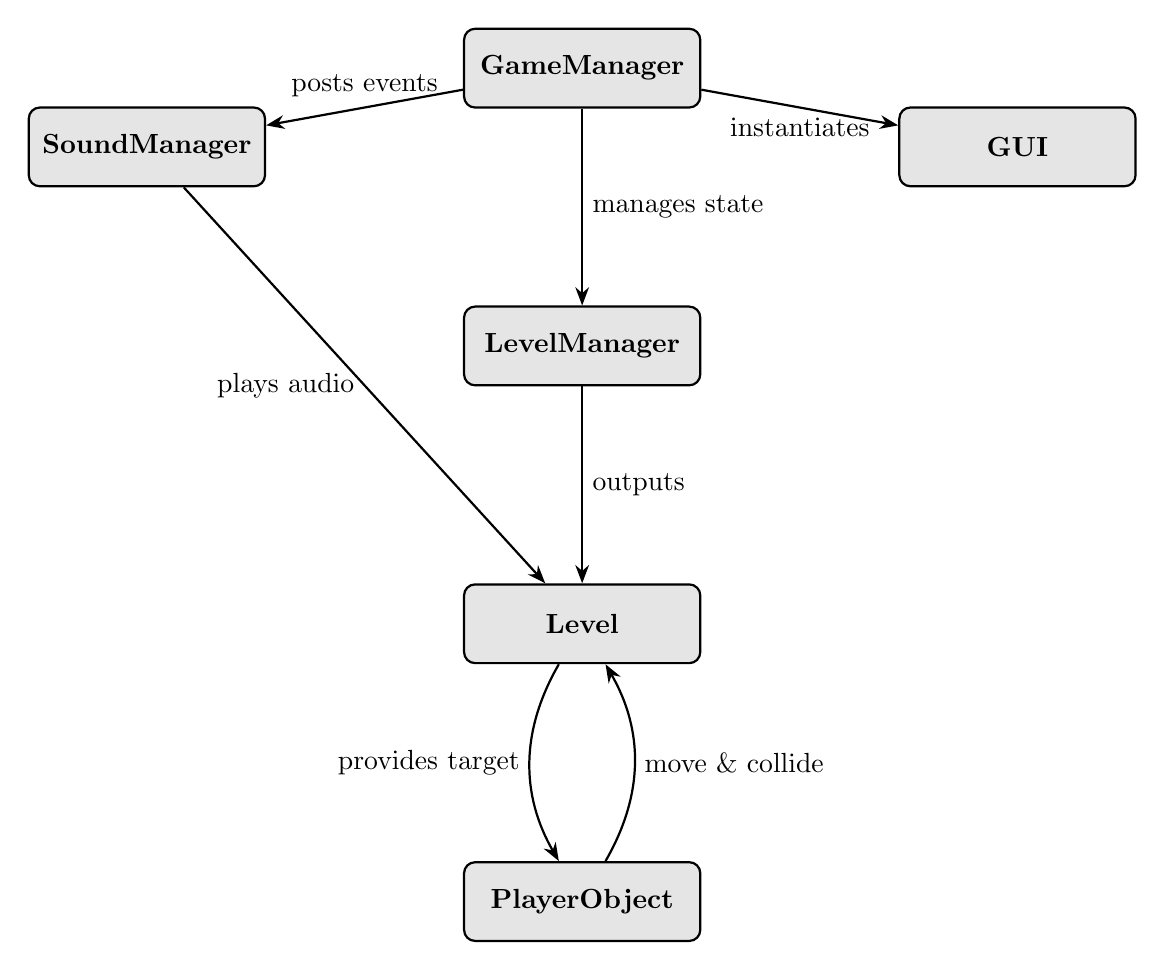
\begin{tikzpicture}[node distance=2.5cm, auto, thick,
	class/.style={rectangle, rounded corners, draw=black, fill=gray!20, minimum width=3cm, minimum height=1cm, align=center}]

	% Nodes
	\node[class] (GM) {\textbf{GameManager}};
	\node[class] (SM) [left=of GM, yshift=-1cm] {\textbf{SoundManager}};
	\node[class] (GUI) [right=of GM, yshift=-1cm] {\textbf{GUI}};
	\node[class] (LevelMgr) [below=of GM] {\textbf{LevelManager}};
	\node[class] (Level) [below=of LevelMgr] {\textbf{Level}};
	\node[class] (Player) [below=of Level] {\textbf{PlayerObject}};

	% Dependencies
	\draw[-Stealth] (GM) to node[above]{posts events} (SM);
	\draw[-Stealth] (GM) to node[right]{manages state} (LevelMgr);
	\draw[-Stealth] (GM) to node[below]{instantiates} (GUI);
	\draw[-Stealth] (LevelMgr) to node[right]{outputs} (Level);
	\draw[-Stealth] (Level) to [bend right=30] node[left]{provides target} (Player);
	\draw[-Stealth] (Player) to [bend right=30] node[right]{move \& collide} (Level);
	\draw[-Stealth] (SM) to node[left]{plays audio} (Level);
	\end{tikzpicture}
	\caption{Core class relationships}
	\label{fig:class_diagram}
\end{figure}
\newpage
% Data Flow
\section{Data Flow Diagram}
\begin{figure}[H]
    \centering
    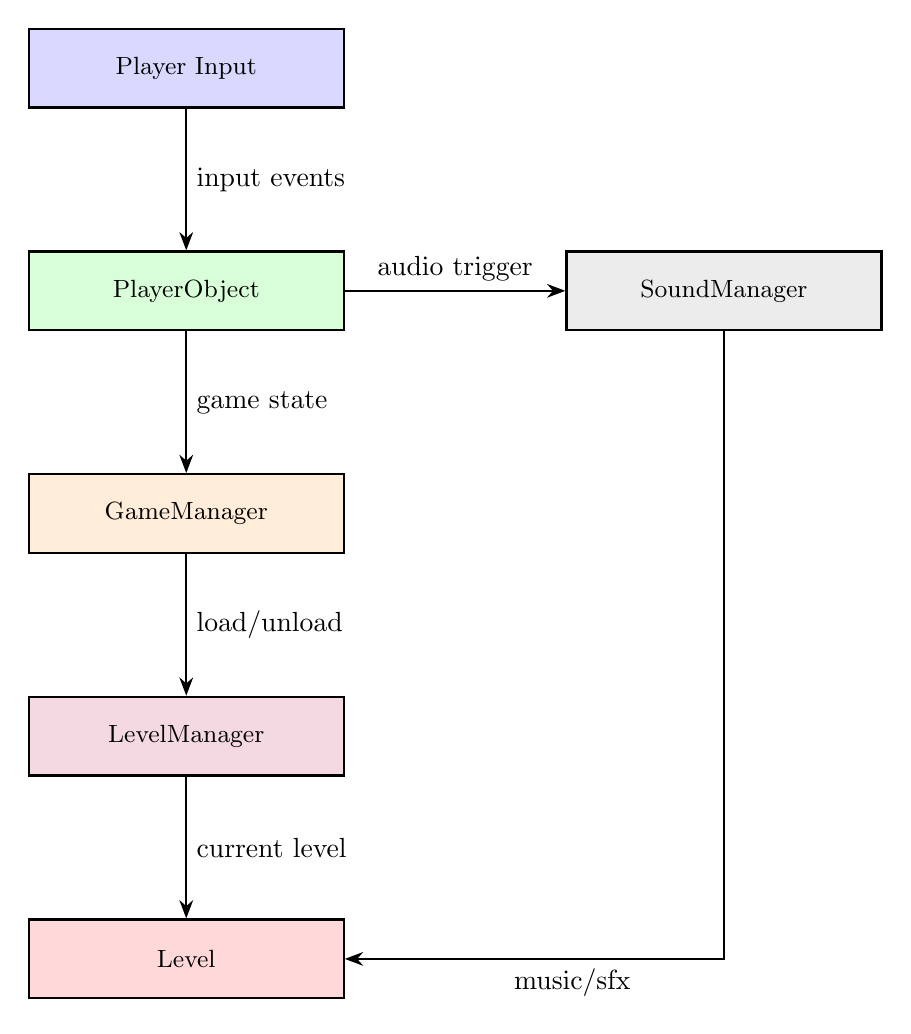
\begin{tikzpicture}[
        node distance=1.8cm, % Vertical spacing
        auto, 
        thick,
        block/.style={rectangle, draw, minimum width=4cm, minimum height=1cm, align=center, font=\small}
    ]
        % Nodes flowing DOWN instead of RIGHT
        \node[block, fill=blue!15] (Input) {Player Input};
        \node[block, fill=green!15, below=of Input] (Player) {PlayerObject};
        \node[block, fill=orange!15, below=of Player] (GameMgr) {GameManager};
        \node[block, fill=purple!15, below=of GameMgr] (LevelMgr) {LevelManager};
        \node[block, fill=red!15, below=of LevelMgr] (Level) {Level};
        
        % SoundManager positioned to the SIDE of the main flow
        \node[block, fill=gray!15, right=of Player, xshift=1cm] (SoundMgr) {SoundManager};

        % Vertical Arrows
        \draw[-Stealth] (Input) -- node[right] {input events} (Player);
        \draw[-Stealth] (Player) -- node[right] {game state} (GameMgr);
        \draw[-Stealth] (GameMgr) -- node[right] {load/unload} (LevelMgr);
        \draw[-Stealth] (LevelMgr) -- node[right] {current level} (Level);

        % Audio Flow (Horizontal then Vertical)
        \draw[-Stealth] (Player) -- node[above] {audio trigger} (SoundMgr);
        
        % Curve the arrow back to the Level at the bottom
        \draw[-Stealth] (SoundMgr.south) |- node[pos=0.7, below] {music/sfx} (Level.east);

    \end{tikzpicture}
    \caption{Runtime data flow (Vertical Architecture)}
    \label{fig:data_flow_vertical}
\end{figure}

\chapter{Detailed Class Descriptions}
\section{GameManager (\texttt{GameManager.cs})}
\begin{enumerate}[label=\alph*)]
	\item\textbf{Singleton pattern}: accessible via \texttt{GameManager.Instance}.
	\item\textbf{State machine}: \texttt{GameState} enum values control flow; events surface transitions.
	\item\textbf{GUI initialization}: asynchronous root injection after a short timer.
	\item\textbf{State change handling}: broadcasts \texttt{GameStateChanged} and updates internal \texttt{CurrentGameState}.
\end{enumerate}

\section{LevelManager (\texttt{LevelManager.cs})}
\begin{enumerate}[label=\alph*)]
	\item\textbf{Level data lookup}: selects packed scenes per \texttt{Difficulty}.
	\item\textbf{Debug reload}: feature active in DEBUG builds, re-instantiates current level.
	\item\textbf{Event hooks}: \texttt{LevelLoaded} and \texttt{LevelUnloaded} for external reactions.
	\item\textbf{Runtime container}: manages \texttt{CurrentLevel} under \texttt{GameSceneRoot}.
\end{enumerate}

\section{Level (\texttt{Level.cs})}
\begin{enumerate}[label=\alph*)]
	\item\textbf{Metadata}: thumbnail, difficulty, distance limits.
	\item\textbf{Music}: audio stream and BPM.
	\item\textbf{Player injection}: on enter tree, grabs \texttt{PlayerObject} child, configures via \texttt{SetLevelBasedVariables}.
	\item\textbf{Progress tracking}: \texttt{UpdateProgress} records travel and painting status.
	\item\textbf{Level completion logic}: \texttt{CheckLevelEnd} compares distance and required progress.
\end{enumerate}

\section{PlayerObject (\texttt{PlayerObject.cs})}
\begin{enumerate}[label=\alph*)]
	\item\textbf{Movement}: constant forward speed, lane switching via gravity flip.
	\item\textbf{Collision handling}: triggers level failure on trap layers or stuck condition.
	\item\textbf{Color selection}: interacts with GUI through input actions.
	\item\textbf{Painting flag}: \texttt{AbleToPaint} indicates when player is in paint mode (placeholder for future integration).
\end{enumerate}

\section{SoundManager (\texttt{SoundManager.cs})}
\begin{enumerate}[label=\alph*)]
	\item\textbf{AudioServer utilization}: underlying Godot audio engine; all \texttt{AudioStreamPlayer}'s are routed through it.
	\item\textbf{Volume management}: master, music, and SFX volumes with linear-to-dB conversion.
	\item\textbf{Playback control}: dedicated methods for music, SFX, track switching.
	\item\textbf{Settings integration}: pulls user preferences from \texttt{SettingsManager} and applies via events.
\end{enumerate}

% Future Design
\chapter{Future Extensions}
\section{BPM Synchronization}
\begin{itemize}[noitemsep]
	\item The current \texttt{Level} stores \texttt{MusicBPM}, but no runtime logic ties paint updates to beat intervals.
	\item Proposed design: a BPM timer node---\texttt{BpmClock.cs}---subscribes to level start; emits \texttt{Beat} events derived from \texttt{MusicBPM}. Components such as \texttt{Renderer} would listen to these events and sync brush strokes.
	\item Interaction with \texttt{AudioServer}: use \texttt{AudioServer.get\_stream\_playback\_position()} to fetch exact sample position for sub-beat precision.
\end{itemize}

\section{Painting Mesh Generation}
\begin{itemize}[noitemsep]
	\item Current code reserves a \texttt{PlayerObject.AbleToPaint} flag but no mesh creation.
	\item Suggested architecture: a \texttt{MeshBuilder} class that consumes player positions over time, generates segmented polyline meshes and uploads them to a \texttt{MeshInstance2D}. The MeshBuilder would interface with the Level to record progress.
	\item Future audio coupling: passing paint events to \texttt{SoundManager} for beat-synchronized effects.
\end{itemize}

\newpage
% \bibliographystyle{plain}
% \bibliography{references}

\end{document}
